\section{Background and Motivation}
\label{sec:background_motivation}

In this section we present the characteristics of video analytics pipelines, providing motivation for integrating mobile video sources into the analytics architecture. We then present the key differences between fixed and mobile cameras, highlighting the challenges that we face when we integrate different types of cameras into such systems.

\subsection{Live Video Analytics}
% In this subsection we present the general characteristics of video analytics and types of choices we can take to make them function.

% \begin{figure}
%     \centering
%     \begin{subfigure}[t]{0.57\linewidth}
%         \centering
%         \includegraphics[width=\linewidth]{chapters/videojam/images/pipelines.pdf}
%         \caption{Applications use different modules depending on the source.}
%         \label{fig:pipelines}
%     \end{subfigure}
%     \hfill
%     \begin{subfigure}[t]{0.37\linewidth}
%         \centering
%         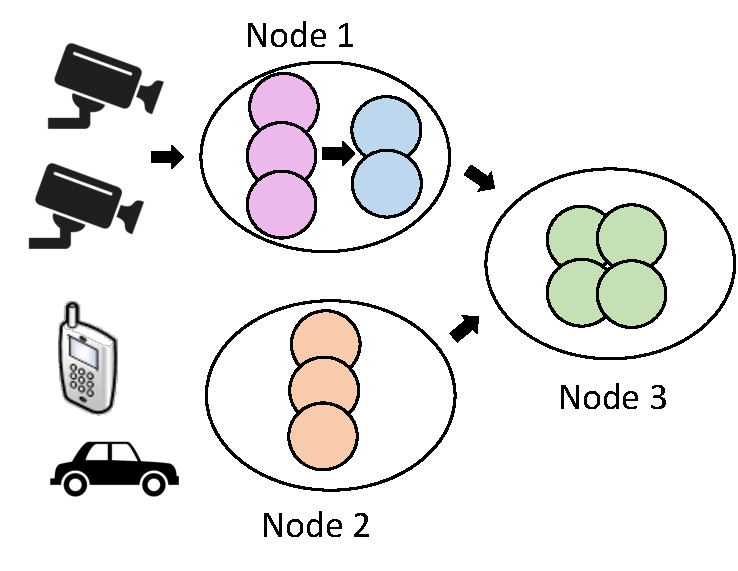
\includegraphics[width=0.8\linewidth]{chapters/videojam/images/dep_example.pdf}
%         \caption{The orchestration determines where to deploy replicas of each module.}
%         \label{fig:dep_example}
%     \end{subfigure}
%     \caption{The characteristics of live video analytics.\fb{I am not sure how needed this figure is or how to adapt it} \sj{The figure quality is quite poor as well.}}
%     \label{fig:video_analytics}
% \end{figure}

\begin{figure}[t]
    \centering
     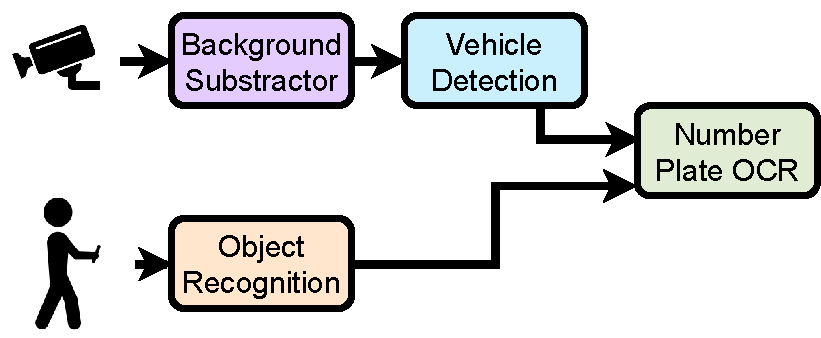
\includegraphics[width=0.75\linewidth]{chapters/videojam/images/video_analytics.pdf}
    \caption{The functions composing a vehicles' number plate detection application pipeline. Different sources require different processing functions.}
    \label{fig:video_analytics}
\end{figure}

% Paragraph on a high level description of video analytics and their applications
Live video analytics center around analyzing video camera streams in real-time, using algorithmic and computer vision techniques to extract valuable information. Incoming frames traverse a series of modules (or \textit{functions}) that perform different tasks, such as object detection, classification, and tracking. These functions are combined into a pipeline, conventionally represented by a directed acyclic graph, where the output of one function is the input of the next and the final output depends on the analytics application deployed.~\Cref{fig:video_analytics} shows an example of video analytics pipelines for a typical traffic control application: vehicles' number plate detection.

% Paragraph on the general structure of video analytics pipelines
Historically, video analytics research has focused its attention on the placement problem occurring at deployment time. Deploying a video analytics application involves taking an orchestration decision of where to place the instances of the application's pipeline. Placement decisions are taken based on the available resources in the compute infrastructure and the workload generated by available cameras. Early work on video analytics focused on how to efficiently transmit video traffic to centralized clouds for processing~\cite{ao2018sprocket,zhang2017live,fouladi2017encoding}. Yet, while centralized datacenters offer unbounded compute resources, transporting the increasing amounts of video streams to these locations can result in network bottlenecks, requiring either to preprocess video frames on premises~\cite{chen2015glimpse,hung2018videoedge} or to reduce the quality of the video transported~\cite{pakha2018reinventing}, potentially affecting the performance of deployed applications.

% Paragraph on the different choices we can take to make them function
To combat these challenges, recent work has focused on deploying video analytics pipelines at the edge of the network~\cite{zeng2020distream,jiang2018chameleon,zhang2019hetero}. These approaches aim to take advantage of compute resources deployed close to video cameras and bypass the transmission to remote locations. However, edge compute devices are often co-located with the existing network equipment and deploy limited computational resources. As a result, they can rapidly become overloaded by incoming video frames causing data loss and reduced accuracy. To address this challenge, different solutions have been proposed to distribute the workload across locations. For example, Distream~\cite{zeng2020distream} exploits the inherent load dynamics present in video flows to split the processing pipeline between two hierarchical locations, \ie, the camera and the edge compute machine. Chameleon~\cite{jiang2018chameleon} instead optimizes the pipelines configuration based on temporal and spatial predictions on the contents of camera sources. 

Yet, all these architectures assume that video flows are generated from fixed cameras (\eg, traffic cameras deployed at street corners) and that their workflows present predictable patterns allowing reconfiguration decisions to be taken at longer timescales, for example when traffic conditions change during the day due to commute patterns. However, mobile cameras have become pervasive in the last decade. Mobile devices, from smartphones to cars and drones all come equipped with high quality camera sensors. These cameras often have the unique advantage of being in the right place at the right time, offering the potential to enhance existing architectures and improve application performance. Unfortunately, video feeds generated by mobile cameras are fundamentally different from fixed camera ones, posing unique challenges into the path for their integration. 


\subsection{Challenges in Incorporating Mobile Cameras}

\begin{figure}
    \centering
    \begin{subfigure}[t]{0.47\linewidth}
        \centering
        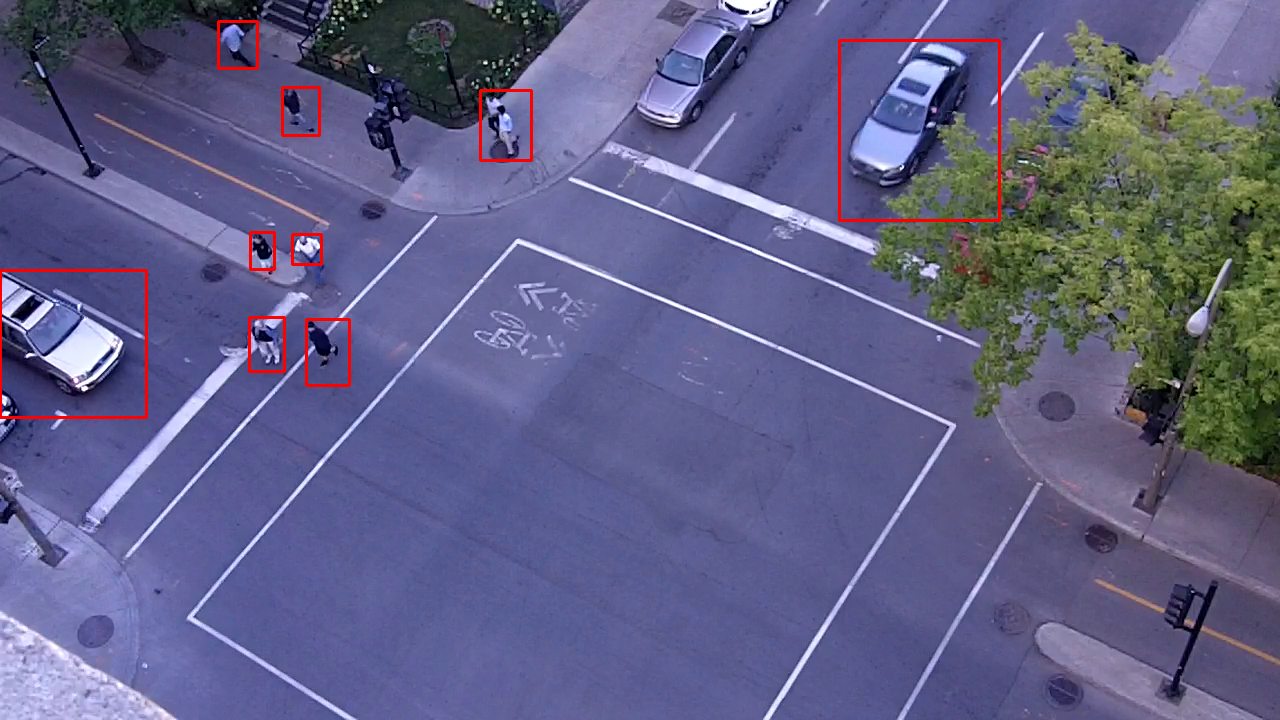
\includegraphics[width=\linewidth]{chapters/videojam/images/fixed_camera_bg_subtractor1003.png}
        \caption{Fixed camera with background subtractor.}
        \label{fig:fixed}
    \end{subfigure}
    \hfill
    \begin{subfigure}[t]{0.47\linewidth}
        \centering
        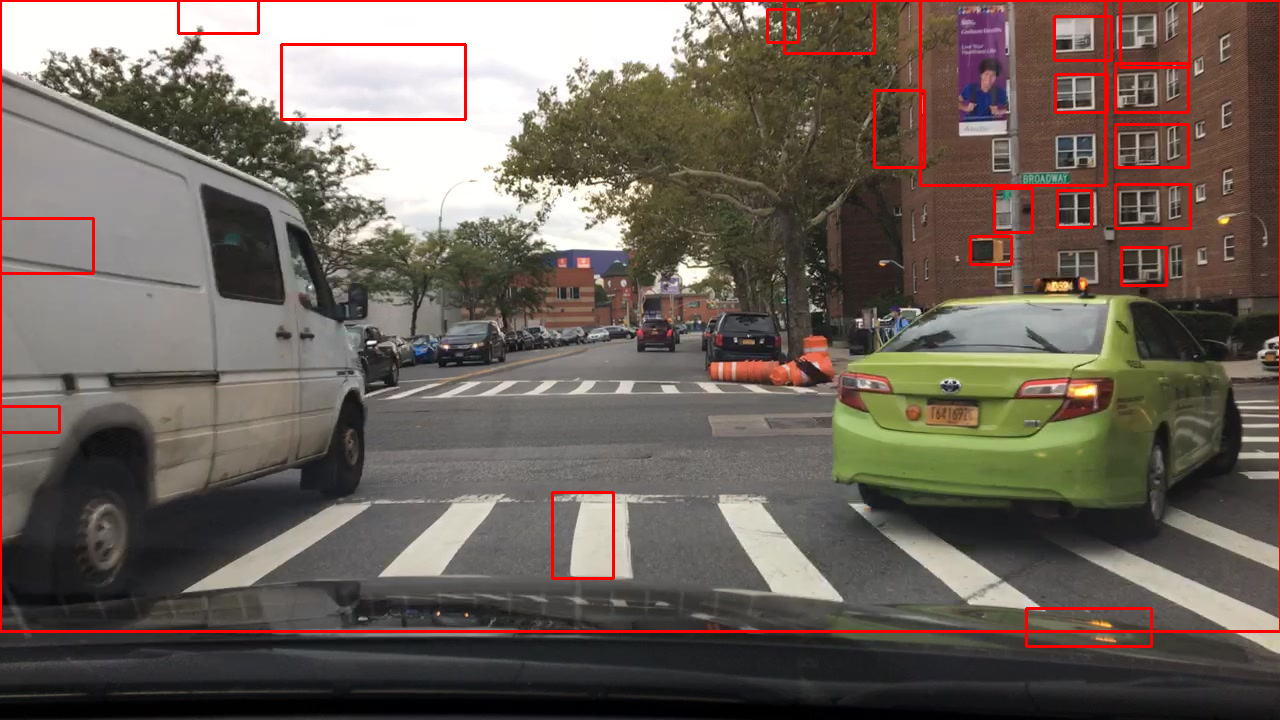
\includegraphics[width=\linewidth]{chapters/videojam/images/mobile_camera_bg_subtractor.png}
        \caption{Mobile camera with background subtractor.}
        \label{fig:mobile}
    \end{subfigure}
    \caption{A comparative example on the performance of background substractor functions on fixed and mobile cameras.}
    \label{fig:backgroung_subtractor}
\end{figure}


Mobile cameras bring the advantage of providing a unique perspective on the captured scenes. They can be in the right place at the right time, capturing scenes that would be otherwise invisible from fixed cameras. However, this benefit comes at the implicit cost of having to handle fundamentally different dynamics. Mobile cameras are constantly moving, capturing new scenes; they can appear and disappear from a deployment; and the scenes they capture can vary more rapidly than for fixed cameras. For these reasons, the differences between fixed and mobile cameras can greatly impact the deployment choices of a video analytics pipeline architecture that aims to process their video feeds. With the goal of designing a video analytics architecture that can handle both fixed and mobile cameras, we identify three core challenges that arise from the coexistence of these cameras in the same deployment.

%This discusses that while previous work uses traffic predict performance profiles, it is not enough to correctly balance the load in the presence of mobile cameras because they come and go.
\paragraph{Challenge \#1: Heterogeneous performance profiles.} 
The majority of existing video analytics solutions~\cite{jiang2018chameleon} assume the homogeneity in the performance of the processing components deployed. Distream~\cite{zeng2020distream} relaxes this assumption by considering the presence of heterogeneous processing devices and accounts for this disparity in implementing load balancing policies within its architecture. However, mobile cameras are inherently in constant movement, quickly capturing new scenes. This makes the processing pipelines that are effective for fixed cameras ineffective for mobile cameras.  

To exemplify the difference between fixed and mobile cameras, we consider a vehicles' number plate detection application. The goal of this application consists of detecting vehicles from a camera frame using a vehicle detection module and extract their number plate via an Optical Character Recognition (OCR) module. To lighten the load of the processing pipeline, the first step involves isolating objects in the frame to limit vehicle detection executions solely on cropped images~\cite{zeng2020distream}. This is typically done using a background subtractor module that compares the current frame with a background model and outputs a mask of the foreground objects~\cite{zeng2020distream}.~\Cref{fig:fixed} shows the output of a background subtractor module applied to a fixed camera frame. We observe that the background subtractor is able to isolate the moving objects in the frame while still objects (\eg, parked cars) are not detected as they are still in the frame. Unfortunately, while the application of a background subtractor is effective for fixed camera streams, the same pipeline becomes ineffective for mobile cameras. By nature, mobile cameras are constantly moving, capturing new scenes. As a consequence, when applied to a moving subject, the subtractor model is not capable of adapting to new scenes, causing erroneous detections or, in the worst case, detecting the entire frame as foreground (as shown in~\Cref{fig:mobile}).

% . shows
% the output of a background subtractor module applied to a mobile camera frame
% where the vehicles in the frame are not detected while other elements (\eg, the
% windows of the building) are. This makes it impossible to isolate the moving
% objects in the frame, forcing the deployment of more expensive object detection modules to process the entire frame. 

\begin{figure}
    \centering
    \begin{subfigure}[t]{0.47\linewidth}
        \centering
        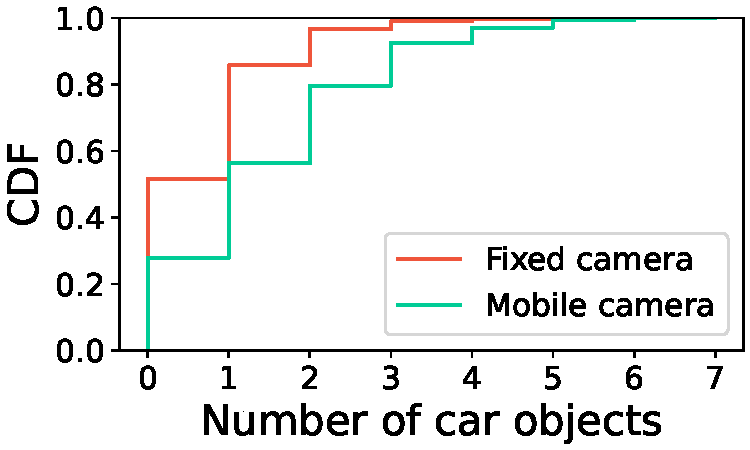
\includegraphics[width=\linewidth]{chapters/videojam/images/fixed_and_mobile_camera_output_filtered.pdf}
        \caption{Number of detected vehicles.}
    \end{subfigure}
    \hfill
    \begin{subfigure}[t]{0.47\linewidth}
        \centering
        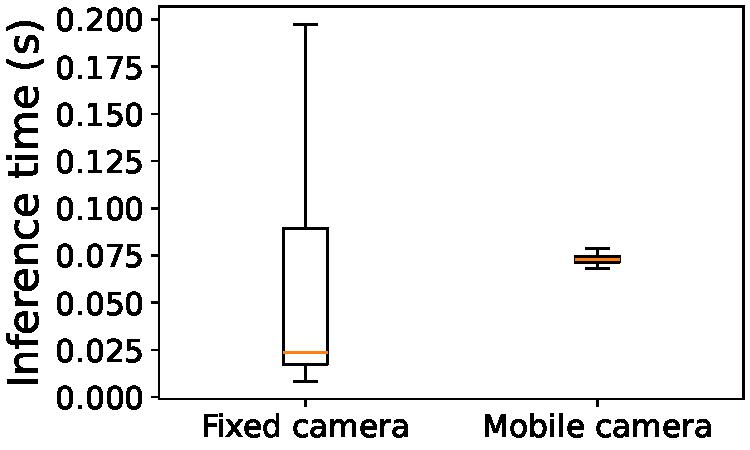
\includegraphics[width=\linewidth]{chapters/videojam/images/inference_times.pdf}
        \caption{Inference time.}
    \end{subfigure}
    \caption{Vehicle detection performance for fixed (background substractor + detection) vs mobile (YOLOv5) cameras.}
    \label{fig:mobile_v_fixed}
\end{figure}

To compensate for the degraded performance of the background substractor module, existing solutions tailored for mobile cameras~\cite{qiu2018kestrel,he2021real} replace the early stages of the pipeline with an object recognition module (\eg, YOLO~\cite{jocher2020yolov5}) that is capable of detecting and classifying objects in the frame in a single operation. However, this comes at a price, as detection models are more resource-intensive, especially for scenarios where no object is in the frame.~\Cref{fig:mobile_v_fixed} shows the performance difference between the two approaches on two selected videos, a fixed and mobile one. We observe that, while the number of detected vehicles is relatively similar across videos, the characteristics of the inference times for the two approaches highly varies depending on the processed frame. In fact, while YOLO achieves consistent results due to its single-pass nature, the performance of the combination of background subtractor and vehicle detection varies according to the number of vehicles present in the frame. Ultimately, this leads to the conclusion that the two approaches should not be treated as interchangeable and that the choice of the pipeline to deploy should be tailored to the video source type.

%This discusses the fact that while previous work aims to balance the load across clusters, it is not enough to balance the load, the presence of diverse pipelines requires different load balancing policies across difference locations.
\paragraph{Challenge \#2: Highly variable workloads.} 
Previous work has highlighted how video camera feeds differ in the amount of objects of interest they capture depending on their deployment location (\eg, a building entrance vs. an emergency exit) and the time of capture (\eg, at night vs during the day)~\cite{yildiz2013optimal,guo2021crossroi}. These differences generate variability in the workload that the video analytics pipeline needs to process and have been exploited to design more efficient processing pipelines~\cite{jiang2018chameleon,zeng2020distream}. Distream~\cite{zeng2020distream} proposed to exploit this variability to dynamically balance the workloads across processing clusters, taking advantage of periods of lower usage from some nodes in the architecture to support overloaded ones. Their solution achieves this through the use of two main design elements: (i) A cross-device workload balancer that takes the cross-camera workload correlations and the heterogeneous compute capabilities of smart cameras and edge clusters to optimize cross-camera workload balancing via an optimization problem; and (ii) a workload adaption controller which triggers the cross-camera workload balancer when cross-camera workload imbalance is detected. 

Unfortunately, this approach assumes that workloads have predictable profiles, either due to the cameras' relative locations, their time of capture~\cite{jiang2018chameleon}, or, more generally, by training a prediction model based on previous patterns~\cite{zeng2020distream}. However, the introduction of mobile cameras generates a new level of variability in the workload that is not easily predictable. First, mobile cameras constantly vary their point of observation and might capture different scenes at different instances in time. Second, the inherent moving nature of mobile cameras causes them to appear or disappear from the deployment, generating sudden changes in the workload that the video analytics pipeline needs to process. Overall, relying on long term prediction models to infer incoming load is not sufficient, or even potentially counter-productive, to correctly balance the load in the presence of mobile cameras.

\begin{figure}
    \centering
    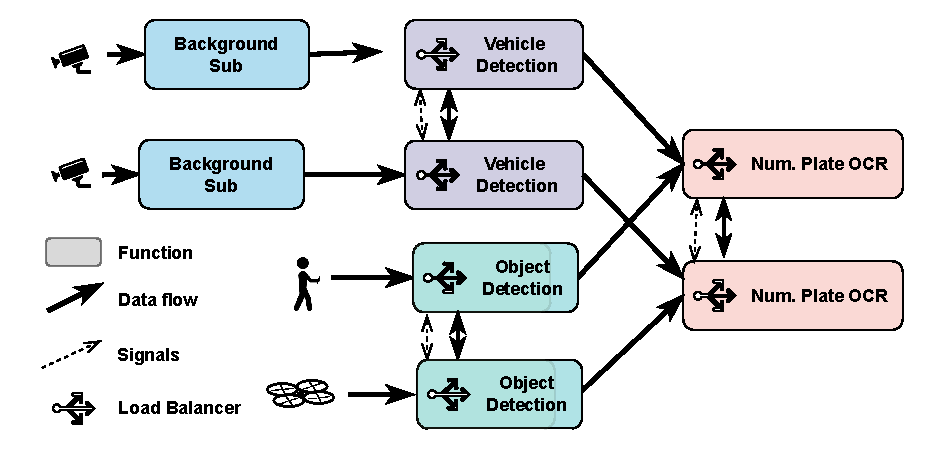
\includegraphics[width=\linewidth]{chapters/videojam/images/architecture.pdf}
    \caption{VideoJam architecture.}
    \label{fig:architecture}
\end{figure}

%This discusses how ultimately we can focus on the previous two, but if the configuration changes, we are screwed. We need an online approach. In particular, there can be a change in in number 
\paragraph{Challenge \#3: Varying configurations.} Early work in video analytics focused on the problem of optimizing the placement in the infrastructure of the functions that belong to the processing pipelines. The placement decisions behind this optimization are conventionally driven by the available resources in the compute infrastructure, \ie, the number of available servers or GPUs, and the workload generated by available cameras, \ie, the number of camera flows to process~\cite{ao2018sprocket,zhang2017live,fouladi2017encoding}. Due to the overhead incurred, changes in the deployment configuration, such as the addition or removal of processing components, occur a longer time scales due long term pattern shifts (\eg, day vs night scenes)~\cite{jiang2018chameleon,zeng2020distream}. However, the presence of mobile cameras introduces a new level of dynamism in the deployment that has yet to be accounted for. Mobile cameras can appear or disappear from the deployment, and the processing pipeline needs to be able to adapt to these changes without requiring a complete reboot of the processing pipelines. Reboots occur when new containers are instantiated or, depending on the load balancing solution, to change load balancing policies. The first point is particularly problematic, as starting up or transferring containers can lead to long delays, causing the loss of frames that could otherwise have been processed. This introduces the need for an online approach to load balancing that can adapt to changes in the deployment configuration, such as the addition or removal of processing components, without requiring any hard reboots and quickly adapting, in less than a few seconds, to the incurred changes.


To address the challenges identified, we present in the following section VideoJam, a live video analytics solution aimed at (i) supporting the coexistence of fixed and moving cameras within the same processing pipeline; (ii) combining horizontal distribution and function-based load balancing, powered by short-term predictions of incoming loads.